%!TeX encoding = UTF-8
%!TeX program = xelatex
\documentclass[notheorems, aspectratio=54]{beamer}
% aspectratio: 1610, 149, 54, 43(default), 32

\usepackage{latexsym}
\usepackage{amsmath,amssymb}
\usepackage{mathtools}
\usepackage{color,xcolor}
\usepackage{graphicx}
\usepackage{algorithm}
\usepackage{amsthm}
\usepackage{lmodern} % 解决 font warning
% \usepackage[UTF8]{ctex}
\usepackage{animate} % insert gif

\usepackage{lipsum} % To generate test text 
\usepackage{ulem} % 下划线,波浪线

\usepackage{listings} % display code on slides; don't forget [fragile] option after \begin{frame}
\usepackage{verbatim}
\makeatletter
\def\verbatim@font{\tiny\ttfamily}
\makeatother

% ----------------------------------------------
% tikx
\usepackage{framed}
\usepackage{tikz}
\usepackage{pgf}
\usetikzlibrary{calc,trees,positioning,arrows,chains,shapes.geometric,%
    decorations.pathreplacing,decorations.pathmorphing,shapes,%
    matrix,shapes.symbols}
\pgfmathsetseed{1} % To have predictable results
% Define a background layer, in which the parchment shape is drawn
\pgfdeclarelayer{background}
\pgfsetlayers{background,main}

\definecolor{AmethystPurple}{HTML}{AEAEDF}
% define styles for the normal border and the torn border
\tikzset{
  normal border/.style={AmethystPurple, decorate, 
     decoration={random steps, segment length=2.5cm, amplitude=.7mm}},
  torn border/.style={AmethystPurple, decorate, 
     decoration={random steps, segment length=.5cm, amplitude=1.7mm}}}

% Macro to draw the shape behind the text, when it fits completly in the
% page
\def\parchmentframe#1{
\tikz{
  \node[inner sep=1.5em] (A) {#1};  % Draw the text of the node
  \begin{pgfonlayer}{background}  % Draw the shape behind
  \fill[normal border] 
        (A.south east) -- (A.south west) -- 
        (A.north west) -- (A.north east) -- cycle;
  \end{pgfonlayer}}}

% Macro to draw the shape, when the text will continue in next page
\def\parchmentframetop#1{
\tikz{
  \node[inner sep=2em] (A) {#1};    % Draw the text of the node
  \begin{pgfonlayer}{background}    
  \fill[normal border]              % Draw the ``complete shape'' behind
        (A.south east) -- (A.south west) -- 
        (A.north west) -- (A.north east) -- cycle;
  \fill[torn border]                % Add the torn lower border
        ($(A.south east)-(0,.2)$) -- ($(A.south west)-(0,.2)$) -- 
        ($(A.south west)+(0,.2)$) -- ($(A.south east)+(0,.2)$) -- cycle;
  \end{pgfonlayer}}}

% Macro to draw the shape, when the text continues from previous page
\def\parchmentframebottom#1{
\tikz{
  \node[inner sep=2em] (A) {#1};   % Draw the text of the node
  \begin{pgfonlayer}{background}   
  \fill[normal border]             % Draw the ``complete shape'' behind
        (A.south east) -- (A.south west) -- 
        (A.north west) -- (A.north east) -- cycle;
  \fill[torn border]               % Add the torn upper border
        ($(A.north east)-(0,.2)$) -- ($(A.north west)-(0,.2)$) -- 
        ($(A.north west)+(0,.2)$) -- ($(A.north east)+(0,.2)$) -- cycle;
  \end{pgfonlayer}}}

% Macro to draw the shape, when both the text continues from previous page
% and it will continue in next page
\def\parchmentframemiddle#1{
\tikz{
  \node[inner sep=2em] (A) {#1};   % Draw the text of the node
  \begin{pgfonlayer}{background}   
  \fill[normal border]             % Draw the ``complete shape'' behind
        (A.south east) -- (A.south west) -- 
        (A.north west) -- (A.north east) -- cycle;
  \fill[torn border]               % Add the torn lower border
        ($(A.south east)-(0,.2)$) -- ($(A.south west)-(0,.2)$) -- 
        ($(A.south west)+(0,.2)$) -- ($(A.south east)+(0,.2)$) -- cycle;
  \fill[torn border]               % Add the torn upper border
        ($(A.north east)-(0,.2)$) -- ($(A.north west)-(0,.2)$) -- 
        ($(A.north west)+(0,.2)$) -- ($(A.north east)+(0,.2)$) -- cycle;
  \end{pgfonlayer}}}

% Define the environment which puts the frame
% In this case, the environment also accepts an argument with an optional
% title (which defaults to ``Example'', which is typeset in a box overlaid
% on the top border
\newenvironment{parchment}[1][Example]{%
  \def\FrameCommand{\parchmentframe}%
  \def\FirstFrameCommand{\parchmentframetop}%
  \def\LastFrameCommand{\parchmentframebottom}%
  \def\MidFrameCommand{\parchmentframemiddle}%
  \vskip\baselineskip
  \MakeFramed {\FrameRestore}
  \noindent\tikz\node[inner sep=1ex, draw=black!20,fill=AmethystPurple, 
          anchor=west, overlay] at (0em, 1em) {\sffamily#1};\par}%
{\endMakeFramed}

% ----------------------------------------------

\mode<presentation>{
    \usetheme{Berkeley}
    % Boadilla CambridgeUS
    % default Antibes Berlin Copenhagen
    % Madrid Montpelier Ilmenau Malmoe
    % Berkeley Singapore Warsaw
    \usecolortheme{dolphin}
    % beetle, beaver, orchid, whale, dolphin
    \useoutertheme{infolines}
    % infolines miniframes shadow sidebar smoothbars smoothtree split tree
    \useinnertheme{circles}
    % circles, rectanges, rounded, inmargin
}
% 设置 block 颜色
\setbeamercolor{block title}{bg=AmethystPurple,fg=white}

\newcommand{\reditem}[1]{\setbeamercolor{item}{fg=red}\item #1}

% 缩放公式大小
\newcommand*{\Scale}[2][4]{\scalebox{#1}{\ensuremath{#2}}}

% 解决 font warning
\renewcommand\textbullet{\ensuremath{\bullet}}

% verbatim


% ---------------------------------------------------------------------
% flow chart
\tikzset{
    >=stealth',
    punktchain/.style={
        rectangle, 
        rounded corners, 
        % fill=black!10,
        draw=white, very thick,
        text width=6em,
        minimum height=2em, 
        text centered, 
        on chain
    },
    largepunktchain/.style={
        rectangle,
        rounded corners,
        draw=white, very thick,
        text width=10em,
        minimum height=2em,
        on chain
    },
    line/.style={draw, thick, <-},
    element/.style={
        tape,
        top color=white,
        bottom color=blue!50!black!60!,
        minimum width=6em,
        draw=blue!40!black!90, very thick,
        text width=6em, 
        minimum height=2em, 
        text centered, 
        on chain
    },
    every join/.style={->, thick,shorten >=1pt},
    decoration={brace},
    tuborg/.style={decorate},
    tubnode/.style={midway, right=2pt},
    font={\fontsize{10pt}{12}\selectfont},
}
% ---------------------------------------------------------------------

% code setting
\lstset{
    language=C++,
    basicstyle=\ttfamily\footnotesize,
    keywordstyle=\color{red},
    breaklines=true,
    xleftmargin=2em,
    numbers=left,
    numberstyle=\color[RGB]{222,155,81},
    frame=leftline,
    tabsize=4,
    breakatwhitespace=false,
    showspaces=false,               
    showstringspaces=false,
    showtabs=false,
    morekeywords={Str, Num, List},
}

% ---------------------------------------------------------------------

%% preamble
\title[Big Data Analysis In ACCRE]{Big Data Analysis in ACCRE}
\subtitle{Report on Learning Big Data Analysis: I}
\author{Fenglai Liu}
\institute[ACCRE]{fenglai@accre.vanderbilt.edu}

% -------------------------------------------------------------

\begin{document}

%% title frame
\begin{frame}
    \titlepage
\end{frame}

\section{Introduction}
\subsection{General Thoughts about My Future Role}
\begin{frame}
%    \frametitle{}

\begin{block}{What can I do as an application developer in ACCRE for big data analysis?}
\begin{itemize}
 \item Teaching;
 \item Helping people solving programming problems on big data;
 \item Helping people on using the cluster for big data analysis
\end{itemize}
\end{block}

 As a software developer the following points on the big data analysis interest me:
\begin{itemize}
 \item What is the best way to understand big data analysis? 
 \item How to understand the difference and similarity between the big data analysis and 
 traditional HPC programming project?
\end{itemize}

\end{frame}

% -------------------------------------------------------------

\begin{frame}
%    \frametitle{}

More specifically, I have the following questions while learning the big data analysis:

\begin{description}
 \item [Data]
 \begin{itemize}
  \item What kind of level of data is ``big data'' and can be benefit from big data analysis?
  \item Does big data analysis can be applied for all formats of data?
  \item What kind of ``data'' projects can be benefit from the big data analysis?
 \end{itemize}
  \item [Tools]
 \begin{itemize}
  \item Comparisons between the big data languages and traditional languages, like Scala VS C++?
  \item Comparisons between the Spark VS openMP, MPI?  
 \end{itemize}
  \item [Project]
 \begin{itemize}
  \item How large for a typical big data project?
  \item Fast development?
  \item Scalability on the cluster?
 \end{itemize}
\end{description} 

\end{frame}

% -------------------------------------------------------------

\begin{frame}
%    \frametitle{}

Upon Will's suggestion, I started the big data analysis journey by beginning from Spark and Scala/Python.
For this report, my talk will be mainly concentrating on this point:
\begin{alertblock}{}
 How can we understand Spark/Scala conceptually? What is the similarities and differences comparing with 
 C++/OpenMP/MPI etc.?
\end{alertblock}


\end{frame}

% -------------------------------------------------------------

%% normal frame
\subsection{General View for Spark}
\begin{frame}
%    \frametitle{}

Spark is a ``framework'' for big data analysis. Why it is called a ``FRAMEWORK''? 
Because it is more than a collection of library:
\begin{description}
 \item [library] Spark can be used a a library for Scala/Python/Java programming languages.
 \item [REPL] Refers to Read-Evaluate-Print-Loop. Spark itself has an inner shell environment, 
 where the user can run the spark API in Scala interactively. PySpark also has REPL function 
 based on Python. 
 \item [flexible extension] further API can be provided through Spark streaming like
 machine learning etc.
\end{description}

One interesting comparison: Spark VS. STL.

\end{frame}
% -------------------------------------------------------------

\begin{frame}


    \begin{block}{How to think about the REPL for Spark?}
    REPL is a good feature for fast development and testing/debugging purpose
    (for example, C++/Java do not have it). It is also 
    good for teaching purpose, too. However, as the code growing and the project 
    becomes more practical, library will be the only 
    choice for production implementation.     
    \end{block}
    
    In conclusion
   \begin{enumerate}
    \item  REPL $\Longrightarrow$ project;
    \item  implementation on local multi-threading env $\Longrightarrow$ practical project on cluster
   \end{enumerate}
      
\end{frame}
% -------------------------------------------------------------

\section{Spark}
\subsection{SparkContext}
\begin{frame}[fragile]
  

   \begin{block}{SparkContext: the main entry point for the Spark functionality.}
   The analog for the SparkContext  is like the MPI\_init function, which initializes the environment for cluster usage. 
   For MPI the configuration information is passed through the MPIEXEC etc. then 
   MPI\_init function can initialize the cluster environment for the application.
   Here SparkContext can use SparkConf
   to set up the configuration information and initializes the Spark.
   \end{block}
   
   Scala example:
   \begin{verbatim}
    import org.apache.spark.SparkConf
    import org.apache.spark.SparkContext

    // define the spark conf
    val conf = new SparkConf()
    conf.setMaster("local[*]")  // using all of available cores 
    conf.setAppName("Spark App test") // set the application name

    // now let's create a new SparkContext according to conf
    val sc = new SparkContext(conf)
   \end{verbatim}     
  
\end{frame}

% -------------------------------------------------------------

\subsection{What is RDD?}
\begin{frame}

 \begin{block}{What is RDD?}
  RDD is simply a collection of readable data records stored in ``MEMORY''(also it can be stored in disk, too). 
  It supports both structured data and unstructured data. 
 \end{block}
 
 \begin{block}{in-memory}
   The most noticeable feature for RDD is that RDD is stored in ``MEMORY''. 
 It's able to transform different dataset like HDFS, Amazon S3, Cassandra etc. 
 (disk-stored) into RDD for Spark use. Secondly, ``in-memory'' also enable the 
 REPL possible. Data processing and data analysis can be performed interactively
 in efficiency. 
 \end{block}

\end{frame}

% -------------------------------------------------------------

\begin{frame}

\begin{figure}
 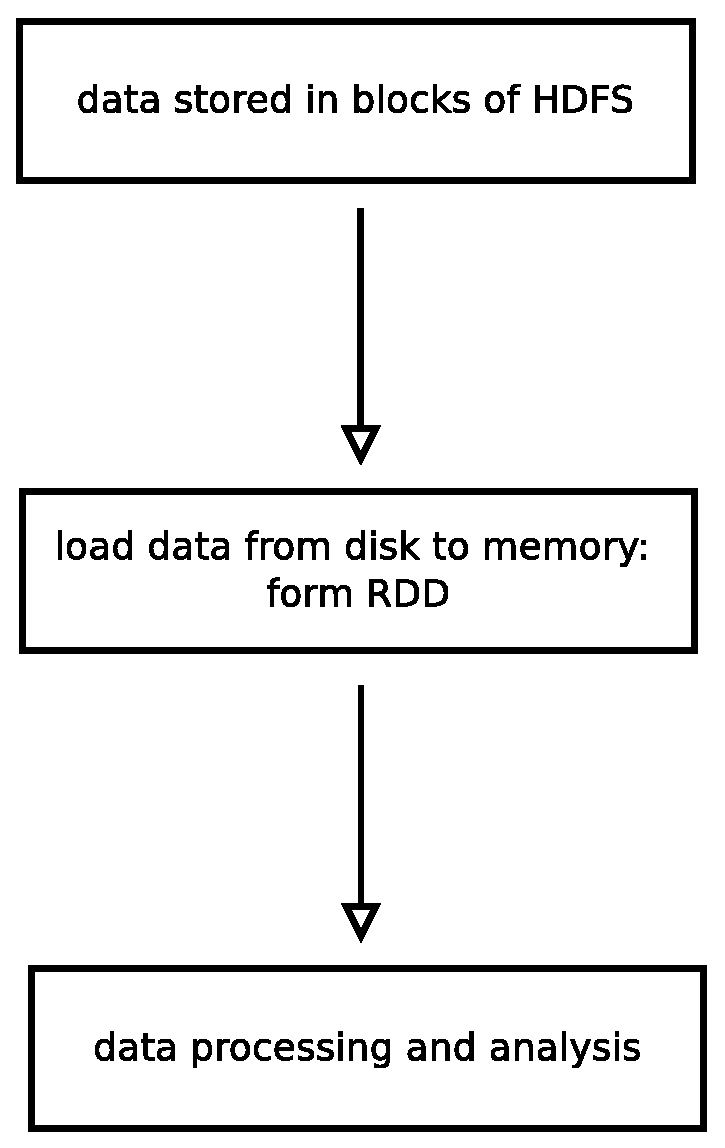
\includegraphics[scale=0.3]{rdd1}
\caption{A simple example demonstrate the relation between RDD and HDFS}
\end{figure} 

\end{frame}


% -------------------------------------------------------------
\subsection{Inside of RDD}
\begin{frame}

An RDD is mainly made up of 4 parts:
\begin{description}
 \item [Partitions] Atomic pieces of the dataset. One or many per RDD.
 \item [Dependencies] Models relationship between this RDD and its partitions with the parent RDDs.
 \item [Function] The function for computing the dataset based on its parent RDDs.
 \item [Metadata] Metadata is about it partitioning scheme and data placement.
\end{description}

\end{frame}


% -------------------------------------------------------------

\begin{frame}

\begin{block}{partition - the unit of RDD}
 The dataset in RDD is in unit of ``partition'' (similar to the blocks in HDFS). 
 Each partition is a slice of dataset, and the whole RDD is stored as 
 many partitions, and these partitions are distributed among the clusters.
\end{block}

\begin{block}{metadata - the information about the partitions}
 Metadata describes the information about the partitions - through the metadata you
 can rebuild the whole dataset from the partitions.
\end{block}

\end{frame}

% -------------------------------------------------------------

\begin{frame}

RDD operations:
\begin{itemize}
 \item transformation: transform the old RDD to new RDD (in other words,
form the children RDD from the parent RDD)
 \item action: operations on the RDD that returns the result (in general, 
 non-RDD return)
\end{itemize}

\begin{alertblock}{data flow is immutable}
 For big data analysis with Spark, the data flow is immutable. Therefore for the data flow we 
 transform it from one type RDD to anther type of RDD. 
\end{alertblock}

\end{frame}

% -------------------------------------------------------------

\begin{frame}

\begin{block}{Functions - describe how we can derive child RDD from parent RDD}
 Functions stores the ``transformation'' between the parent RDD and the child RDD. 
\end{block}

\begin{block}{Dependencies - the information about the partitions}
 Dependencies describe the dependency relations between partitions in child RDD and the partitions in parent RDD. 
 In general, depending on the operations the dependencies could be in ``narrow dependency'' or ``wide dependency''.
\end{block}

\end{frame}

% -------------------------------------------------------------

\begin{frame}

\begin{block}{What is ``Lazy Evaluation'' for RDD?}
 Lazy evaluation is an idea very common in functional programming. It means for an expression, i
 t will be computed when it is really needed (for example, to cache it(save the RDD to the local memory), 
 save the RDD to file on disk, or derive results from the RDD). 
\end{block}

\begin{block}{How the ``Lazy Evaluation'' works in RDD?}
For transformation operations, a child RDD is only generated the ``functions'' and the ``dependencies'' 
so that we know how to compute a child RDD from parent RDD. 
The data slice like partition and metadata is actually not computed until there's 
action operation is needed. In this way, the creation of RDD can be both memory and  CPU efficient.
\end{block}


\end{frame}

% -------------------------------------------------------------

\begin{frame}

\begin{block}{narrow dependency}
 If each of the partitions of an RDDs are created from only one partition of a single RDD, then it is a narrow dependency. 
\end{block}

\begin{block}{wide dependency}
 If a partition in a RDD is created from more than one partition(from same or different RDD), then it is a wide dependency.
\end{block}

the narrow dependency is always good for RDD transformation. Because all of operations can be performed ``locally''. 
However, wide dependency may not be good, since the parent partitions the child RDD depending on may stored in 
a different node. This situation will make the Spark slow in efficiency. 

\end{frame}

% -------------------------------------------------------------

\begin{frame}

\begin{alertblock}{ partition is also the index of parallelism}
 Spark can only run 1 concurrent task for every partition of an RDD, up to the number of cores in your cluster. 
\end{alertblock}

From this feature, we know two points regarding the Spark:
\begin{itemize}
 \item Spark operations are performed in batches, the unit is in partitions. 
 \item locality is important for RDD operations. 
\end{itemize}
A similar example to understand the locality in RDD is the ``false sharing'' in the Multi-threading.

\end{frame}

% -------------------------------------------------------------

\begin{frame}

Two type of partitions in RDD:
\begin{block}{\textbf{Hash type partition}}
 There are two types of partitions in RDD, one is the ``Hash'' type of partition:
 \begin{displaymath}
  \text{(key1,value1)}  \quad \text{(key2,value2)} \quad \text{(key3,value3)}  \quad \cdots
 \end{displaymath}
\end{block}

  \begin{block}{\textbf{range type partition}}
 \begin{displaymath}
  \text{(1,value1)}  \quad \text{(2,value2)} \quad \text{(3,value3)}  \quad \cdots
 \end{displaymath}
\end{block}
 
\end{frame}

% -------------------------------------------------------------
\subsection{Example for Creating RDD}
\begin{frame}[fragile]
  %  \frametitle{How can we improve the diagnosis}

  A simple case that the hash partition is created (rademe.txt):
  \begin{verbatim}
Spark is a fast and general cluster computing system for Big Data. It provides
high-level APIs in Scala, Java, Python, and R, and an optimized engine that
supports general computation graphs for data analysis. It also supports a
rich set of higher-level tools including Spark SQL for SQL and DataFrames,
MLlib for machine learning, GraphX for graph processing,
and Spark Streaming for stream processing.
  \end{verbatim}

\end{frame}

% -------------------------------------------------------------

\begin{frame}[fragile]
  %  \frametitle{How can we improve the diagnosis}

  based on this paragraph we can create a RDD in the Spark-Shell:
  \begin{verbatim}
  scala> val rdd = sc.textFile (“readme.txt”)   
  scala> rdd.partitions.length
res2: Int = 2
scala> rdd.foreachPartition( i => println("each partition content : " + i.toList))
each partition content : List(, Spark is a fast and general cluster computing 
system for Big Data. It provides, high-level APIs in Scala, Java, Python, 
and R, and an optimized engine that, supports general computation graphs 
for data analysis. It also supports a)
each partition content : List(rich set of higher-level tools including 
Spark SQL for SQL and DataFrames, , MLlib for machine learning, GraphX 
for graph processing,, and Spark Streaming for stream processing., )
  \end{verbatim}
So there are two partitions created in this RDD, 
and the whole text is divided into two
segments, and each partition has one segment.

\end{frame}

% -------------------------------------------------------------

\begin{frame}[fragile]

In the above example we convert the data in partition to List, one of the built-in data
structure in Scala, however we can also print it into vector or set etc.:
\begin{verbatim}
scala> rdd.foreachPartition(i => println("partition content " + i.toSet))
partition content Set(higher-level tools including Spark SQL for SQL and DataFrames,, 
MLlib for machine learning, GraphX for graph processing,, and Spark Streaming for 
stream processing., )
partition content Set(, It provides high-level APIs in Scala, Java, Python, and R, , 
and an optimized engine that supports general computation , graphs for data analysis. 
It also supports a rich set of , Spark is a fast and general cluster computing 
system for Big Data. )
\end{verbatim}
\end{frame}


% -------------------------------------------------------------

\begin{frame}[fragile]

another example for RDD:
\begin{verbatim}
 scala> val rdd1 = sc.parallelize(1 to 10, 3)
rdd1: org.apache.spark.rdd.RDD[Int] = ParallelCollectionRDD[7] 
at parallelize at <console>:24

scala> rdd1.foreachPartition(i => println("partition content " + i.toList))
partition content List(4, 5, 6)
partition content List(7, 8, 9, 10)
partition content List(1, 2, 3)
\end{verbatim}

\end{frame}


% -------------------------------------------------------------

\subsection{Flowchart for Big Data Analysis}
\begin{frame}
 %   \frametitle{How can we improve the diagnosis}

 \begin{figure}
 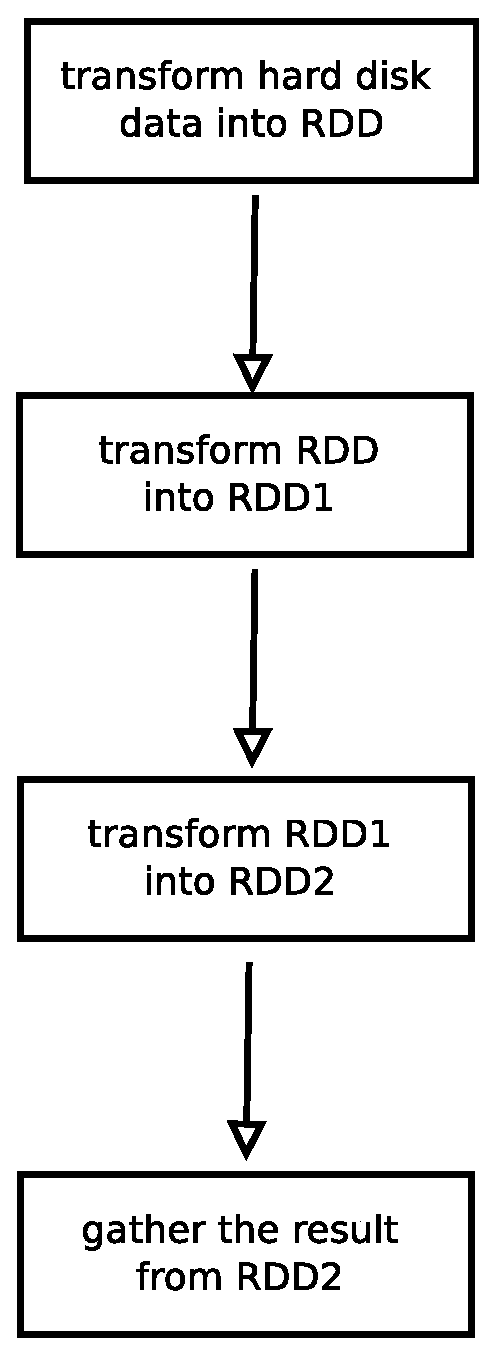
\includegraphics[scale=0.3]{rdd2}
\caption{general view for using Spark in big data analysis}
\end{figure} 

\end{frame}


% -------------------------------------------------------------

\subsection{Transformation Operations on RDD}
\begin{frame}[fragile]

Transformation operations are transforming the RDD into a new RDD. The transformation operations take function as input.
As what we have stated previously, the narrow dependency is the most simplest and efficient operations. Hence let's start
with the narrow transformation operations first.

\begin{block}{map - transforming each element of RDD into a new one (one to one)}
\begin{verbatim}
scala> val a = sc.parallelize(List("dog", "tiger", "lion", "cat", " eagle"), 2)
scala> val b = a.map(x => (x.length, x))  
\end{verbatim}
\end{block}
In this case the passed in list of strings are partitioned into 2 RDDs. For each string in the RDD, through the map operation
each string becomes a tuple (string\_length, string\_content).

\end{frame}

% -------------------------------------------------------------

\begin{frame}[fragile]

\begin{block}{flatMap - transforming each element in RDD into a new set (one to many)}
\begin{verbatim}
scala> val rdd1 = rdd.flatMap(line => line.split(" "))  
\end{verbatim}
\end{block}
In this case the text file inside the rdd is splited into many words by the space, returning to the rdd1. 

\begin{block}{filter - filtering out the elements in RDD depending on some conditions (many to one)}
\begin{verbatim}
scala> val rdd1 = rdd.filter(line => line.split(" ")).filter(line => line == "test")  
\end{verbatim}
\end{block}
In this case the result rdd1 only contains the string of ``test''.

\end{frame}


% -------------------------------------------------------------

\begin{frame}[fragile]

In the above examples, they are all narrow dependency operations - safe, efficient and simple (like embarrassing parallel). 
Now the more difficult model is the wide dependency operations.

\begin{block}{groupByKey - groups all values with respect to a single key}
\begin{verbatim}
scala> val wordFrequencies = x.flatMap(line.split(" ").map(word => (word, 1)).
groupByKey().map((x,y) => (x,sum(y)))
\end{verbatim}
\end{block}


\begin{block}{reducebyKey - counting all of values with respect to a single key}
\begin{verbatim}
scala> val wordFrequencies = x.flatMap(line.split(" ").map(word => (word, 1)).
reduceByKey(()).map((x,y) => (x,sum(y)))
\end{verbatim}
\end{block}
Both of the two examples calculates the word frequencies in the given text file.

\end{frame}

% -------------------------------------------------------------
\subsection{Action Operations on RDD}
\begin{frame}[fragile]

\begin{block}{action operations:}
  Operations on the RDD objects so that to return a non-RDD result. This will cause all of 
  previous lazy evaluated operations put on ``action'' so especially consumes a lot of resource to finish.
\end{block}

\begin{block}{collect - return all the elements of the dataset as an array}
The API of collect function is very simple - it does not need any parameters. However, the action taken by ``collect'' is very 
complicated, it will send all of result RDDs to the master node and transform them into an array. As we all know from HPC, this step
can cause trouble in terms of network and available resources in the cluster.
\end{block}


\begin{block}{reduce - performing operation on all of RDD elements and return a value}
\begin{verbatim}
scala> val x = sc.parallelize(1 to 10, 2)
scala> val y = x.reduce((accum,n) => (accum + n)) 
\end{verbatim}
\end{block}

\end{frame}

% -------------------------------------------------------------
\subsection{Further Thoughts for Spark on Cluster}
\begin{frame}[fragile]

\begin{block}{comparison between applications of Spark and HPC}
 \begin{itemize}
 \item Spark API are all highly abstracted interface, however to properly use them could be a problem;
 \item In applying Spark for big data analysis the troubles usually very similar with HPC programming.
 \item A different case is memory/network overflow occurs more frequently in Spark.
\end{itemize}
\end{block}

A simple case:
\begin{verbatim}
var counter = 0
var rdd = sc.parallelize(data)

// Wrong: Don't do this!!
rdd.foreach(x => counter += x)

println("Counter value: " + counter)
\end{verbatim}

\begin{block}{Why this code piece fails?}
Because counter is only in mater node but not in the worker node! Simiarly to the MPI.
\end{block}

\end{frame}

% -------------------------------------------------------------
\subsection{Subjects for Future Talk}
\begin{frame}

\begin{block}{cluster related topics:}
 \begin{itemize}
 \item Spark job distribution and submission in SparkContext;
 \item Spark partitions shuffle;
 \item Spark DAG (Directed Acyclic Graph);
 \item Spark caching; 
\end{itemize}
\end{block}

\begin{block}{Scala related topics:}
  \begin{itemize}
  \item Spark lineage (due to lazy evaluation);
  \item Data structures (list, set etc.) in Scala used for Spark;
  \item How to use functional programming in Spark?
\end{itemize}
\end{block}

\end{frame}

% -------------------------------------------------------------

\begin{frame}


\begin{block}{Spark features:}
 \begin{itemize}
  \item Spark dataframe;
  \item Spark streaming;
  \item Spark MLlib and Spark SQL etc.
 \end{itemize}

\end{block}

\end{frame}


% -------------------------------------------------------------
\subsection{Future Plan}
\begin{frame}


 \begin{itemize}
 \item Currently I set up a general understanding on the structure of Spark (begin to read the code!); 
 \item Second step, is to plunge into world of Scala to understand more about functional programming (next talk topic, probably on Jan. 3rd);
 \item Thirdly step, return to Spark focusing on the more details than the concepts(the following one/two talks topic);
 \item Final step, for practical projects/teaching (approximately on next March).
\end{itemize}

\end{frame}

\end{document}


